%-----------------------
%       Settings 
%-----------------------
\documentclass[12pt,aspectratio=169]{ctexbeamer}
\setCJKsansfont{FZY3K--GBK1-0}
\usetheme[secheader]{Boadilla} %{Singapore} {Boadilla}
\useoutertheme[subsection=false]{smoothbars}
\usecolortheme{default}
% 修改 itemize 模板,设置负间距
\setbeamertemplate{itemize/enumerate body begin}{\vspace*{-5mm}}
%\addtobeamertemplate{block begin}{\vspace*{-5mm}}
%\addtobeamertemplate{description body begin}{}{\vspace*{-5mm}}
\setbeamertemplate{navigation symbols}{} % delete navigation
\setbeamertemplate{itemize item}{\textcolor{blue}{$\blacksquare$}}
\setbeamertemplate{enumerate item}{\textcolor{blue}{\insertenumlabel.}}
\setbeamertemplate{itemize subitem}{\textcolor{blue}{$\blacksquare$}}
\setbeamertemplate{itemize subsubitem}{\textcolor{blue}{$\blacksquare$}}
\setbeamertemplate{enumerate subitem}{\textcolor{blue}{\insertenumlabel.}}
\setbeamerfont{author}{size=\normalsize}
\setbeamerfont{institute}{size=\footnotesize}
\setbeamerfont{itemize item}{size=\footnotesize}
\setbeamerfont{itemize/enumerate body}{size=\large}
\setbeamerfont{itemize subitem}{size=\scriptsize}
\setbeamerfont{itemize subsubitem}{size=\tiny}
\setbeamerfont{itemize/enumerate subbody}{size=\normalsize}
%{size=\fontsize{14}{17}\selectfont} 
\setbeamerfont{section in toc}{size=\large}
\setbeamerfont{caption}{size=\footnotesize}
\setbeamercolor{mini frame}{fg=blue}
\setbeamercolor{section in head/foot}{fg=blue}
\setbeamercolor{item projected}{bg=lightgray,fg=black}
\setbeamercolor{block title}{bg=lightgray}
\setbeamercolor{block body}{bg=lightgray!400!white!10!}
\setbeamercolor{palette primary}{bg=white,fg=black}
\setbeamercolor{palette secondary}{bg=lightgray!400!white!10!,fg=black}
\setbeamercolor{palette tertiary}{bg=lightgray,fg=black}
\setbeamercolor{palette quaternary}{bg=lightgray,fg=black}
%\setbeamerfont{structure}{size=\large} 
%\setbeamercolor{progressbar}{fg=white,bg=blue}
%\setbeamercolor{smoothbars}{fg=blue,bg=white}
\usepackage{graphicx}
%\usepackage{subcaption}
\usepackage{etoolbox} %用于修改 LaTeX 文档结构、处理列表、管理计数器等功能的命令和工具,如\AtBeginEnvironment
\AtBeginEnvironment{itemize}{\justifying} %缺点是不能递归到sub环境
\AtBeginEnvironment{enumerate}{\justifying} %缺点是不能递归到sub环境
%% 递归设置itemize及其嵌套的子环境为\justifying
%\makeatletter
%\BeforeBeginEnvironment{itemize}{%
	%	\ifnum\@itemdepth >1\relax
	%	\justifying
	%	\fi
	%}
%\makeatother
%% 递归设置enumerate及其嵌套的子环境为\justifying
%\makeatletter
%\BeforeBeginEnvironment{enumerate}{%
	%	\ifnum\@itemdepth >1\relax
	%	\justifying
	%	\fi
	%}
%\makeatother
\usepackage{amsmath}
\usepackage{hyperref}
\usepackage{wrapfig} %图文混排
\usepackage{microtype} %微调单词的间距
\usepackage{multicol} %用于文段平均分
\usepackage{fontspec} %使用TrueType 或 OpenType字体
%\usepackage{mathspec} %使用公式字体
\setmainfont{Palatino Linotype} %使用系统中的Palatino字体
\usepackage{subfig} % Sub-figures
\usepackage{ragged2e} % Auto-line feed
%\usepackage{geometry} % Set layout
\usepackage{apacite} %\bibliographystyle{apacite}
\usepackage{hyperref} %超链接功能
%\usepackage{color}
%\hypersetup{
	%	colorlinks=true,
	%	linkcolor=black,
	%	filecolor=blue,      
	%	urlcolor=blue,
	%	citecolor=cyan,
	%} %改变颜色
\renewcommand{\familydefault}{\rmdefault} %不知道什么问题,只有开了才能显示Palatino字体
\setbeamertemplate{caption}[numbered] % Ordering captions by numbers
\setlength{\abovecaptionskip}{2mm} % Spacing between a figure and its caption adjusted
\AtBeginSection[]
{
	\begin{frame} %[t]%[shrink]
		\frametitle{\makebox[\framewidth]{目录
		\hfill\raisebox{-0.65ex}{\vspace*{10mm}
\includegraphics[height=0.1\textheight]{slogo}\hspace{-4mm}}}}
		\begin{columns}
			\hspace{2cm} % 在这里添加水平间距
			\column{0.5\textwidth}
			\tableofcontents[sections={1-3},currentsection,hideallsubsections]
			
			\column{0.5\textwidth}
			\tableofcontents[sections={4-6},currentsection,hideallsubsections]
		\end{columns}
	\end{frame}
} % Set navigation contents in each section from the start
%\hyphenpenalty=5000 % Justify align
%\tolerance=1000 % Justify align
%\hyphenation{hy-phen-a-tion, A-B-C} % Justify align
%\usepackage{fontspec} % Font package
%\newfontfamily{Georgia} % 这个字体和Boadilla主题冲突了。。。
%\usepackage{fancyhdr} 
%\renewcommand{\headrulewidth}{1mm} %页眉线宽,设为0可以去页眉线
%\renewcommand{\footrulewidth}{1mm} %页脚线宽,设为0可以去页眉线
%			\begin{multicols}{2}
	%	\tableofcontents[currentsection,hideallsubsections]
	%			\end{multicols}
%\frame{\begin{multicols}{2}
		%\end{multicols}}
		%\setbeamertemplate{footline}[frame number]
		%\usepackage{multicol}
		%\usepackage{flushend}	
		
		%-----------------------
		%       Title Information 
		%-----------------------
		
		\title[硕士研究生学位论文答辩]
		{
		\heiti{\normalsize 硕士研究生学位论文答辩}\\
		\vspace{1mm}
		\songti{\textbf{金融创新对中国货币政策传导效率的影响研究}}
		}
%		\subtitle{\textbf{\large 硕士研究生学位论文答辩}}
		\author[202140100058]{} % (optional, for multiple authors)
		%{答辩学生:202140100058 \newline \vspace*{-3mm} \newline 指导老师:XX}
		\institute[]{江西师范大学财政金融学院}
		\date[2024年5月26日] % (optional)
		{2024年5月26日,南昌}
		\vspace*{-5mm}
		\titlegraphic{
\includegraphics[width=18mm]{logo}}
%		\logo{
\includegraphics[height=0.1\textheight]{slogo} \vspace{6cm}}
		
		\begin{document}
			%-----------------------
			%       Make Title 
			%-----------------------
			
			%	\frame{\titlepage}
			\begin{frame}[plain] %start from contents
				\maketitle
%				\vspace*{-5mm}
%				\begin{figure}[htpb]
%					
\includegraphics[width=0.12\textwidth]{logo}
%				\end{figure}
			\end{frame} %start from contents

			%-----------------------
			%       Personal Remarks 
			%-----------------------			
			% \begin{frame}[label=pr]
			% 	\frametitle{\makebox[\framewidth]{重要内容预览
			% 			\hfill\raisebox{-0.65ex}{\vspace*{10mm}
\includegraphics[height=0.1\textheight]{slogo}\hspace{-4mm}}}}
			% 	\begin{itemize}
			% 		\item {研究问题}
			% 		\begin{itemize}
			% 			\justifying
			% 			\item 宏观金融创新对传统货币政策传导渠道的赋能几何,以及对实体经济目标与宏观审慎目标的溢出效果。
			% 			\hyperlink{lr}{\beamergotobutton{跳转}}
			% 		\end{itemize}
			% 		\item {理论缺陷}
			% 		\begin{itemize}
			% 			\justifying
			% 			\item 以金融科技为驱动的金融创新丰富了金融创新的内涵和外延,传统的信息经济学理论无法对金融创新影响逆向选择和道德风险的效果进行简单概括,更难以评价宏观层面对货币政策的作用机制。
			% 			\hyperlink{theo-flaws}{\beamergotobutton{跳转}}
			% 		\end{itemize}
			% 		\item {研究意义}
			% 		\begin{itemize}
			% 			\justifying
			% 			\item \textbf{理论意义:}既有理论提出了纳入“金融稳定”的货币政策规则,本文研究丰富了货币政策传导与金融创新的研究思路,为将来考虑金融创新的“稳定规则”提供支撑。
			% 			\hyperlink{meaning}{\beamergotobutton{跳转}}
			% 		\end{itemize}
			% 		\item {研究思路} \hyperlink{thought}{\beamergotobutton{跳转}}
			% 		\qquad {\footnotesize \textcolor{blue}{$\blacksquare$}} {主要结论} \hyperlink{conclusion}{\beamergotobutton{跳转}}
			% 		\qquad {\footnotesize \textcolor{blue}{$\blacksquare$}} {创新点} \hyperlink{novelty}{\beamergotobutton{跳转}}
			% 	\end{itemize}
			% \end{frame}
			
			%-----------------------
			%       Make Contents 
			%-----------------------
			\begin{frame}
				\frametitle{\makebox[\framewidth]{目录
				\hfill\raisebox{-0.65ex}{\vspace*{10mm}
\includegraphics[height=0.1\textheight]{slogo}\hspace{-4mm}}}}
				\begin{columns}
					\hspace{2cm} % 在这里添加水平间距
					\column{0.5\textwidth}
					\tableofcontents[sections={1-3},hideallsubsections]
					
					\column{0.5\textwidth}
					\tableofcontents[sections={4-6},hideallsubsections]
				\end{columns}
				%\begin{multicols}{2}
				%		\tableofcontents[hideallsubsections]
				%\end{multicols}
				%\restoregeometry
			\end{frame}
			
			%-----------------------
			%       Body
			%-----------------------
			\section{绪论}
			\subsection{研究背景与意义}		
			\begin{frame}[label=meaning]
				\frametitle{\makebox[\framewidth]{1.1研究背景与意义
					\hfill\raisebox{-0.65ex}{\vspace*{10mm}
\includegraphics[height=0.1\textheight]{slogo}\hspace{-4mm}}}}
				\begin{wrapfigure}[9]{r}{5cm}
					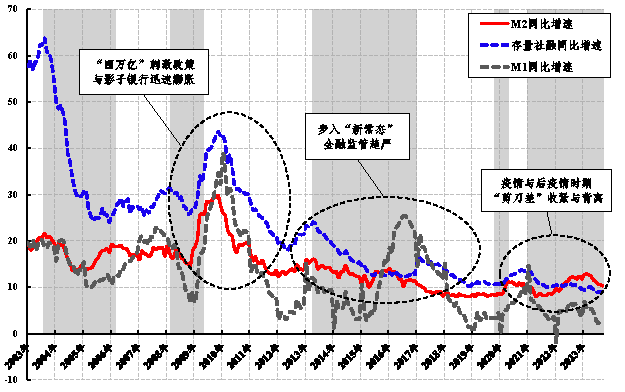
\includegraphics[width=5cm]{figures/fig.1-1}
					\caption{宏观融资需求与流动性变化}
					\label{流动性囤积}
				\end{wrapfigure}
				\vspace*{-3mm}
				\justifying
				\textcolor{blue}{$\blacksquare$} \large 研究背景\\
				\normalsize
				\hspace{2em}
				\textcolor{blue}{1.} \textbf{现实背景:}货币政策传导受阻与“流动性囤积”;\\
				\hspace{2em}
				\textcolor{blue}{2.} \textbf{政策背景:}“完善货币政策传导机制,疏通货币政策传导渠道”;\\
				\hspace{2em}
				\textcolor{blue}{3.} \textbf{现实启示与政策要求:}货币政策、金融稳定与金融创新三者的联系。\\
				\normalsize
				\textcolor{blue}{$\blacksquare$} \large 研究意义 \hyperlink{pr}{\beamergotobutton{}}\\
				\normalsize
				\hspace{2em}
				\textcolor{blue}{1.} 不仅丰富了当前货币政策传导与金融创新的研究思路,还为研究“双支柱”调控的政策溢出提供了有益补充;\\
				\hspace{2em}
				\textcolor{blue}{2.} 进一步探究金融创新赋能传导效应的实际效果,对于疏通货币政策传导渠道以及维护金融稳定,具有十分重要的现实意义与政策内涵。
			\end{frame}
			\subsection{文献综述}
			\begin{frame}[label=lr]
				\frametitle{\makebox[\framewidth]{1.2文献综述 
					\hfill\raisebox{-0.65ex}{\vspace*{10mm}
\includegraphics[height=0.1\textheight]{slogo}\hspace{-4mm}}}}
				\begin{itemize}
					\item 文献梳理的三大视角\\
					\normalsize 多重视角下的货币政策传导;货币政策影响金融稳定目标;金融创新冲击货币政策体系
					\item \large 文献评述
					\hyperlink{pr}{\beamergotobutton{}}
					\begin{enumerate}
						\justifying
						\item \textbf{已有贡献:}以上研究基于货币政策框架转型的不同视角,开展了政策规则、政策工具与目标、传导渠道,以及金融创新与金融稳定等的研究前沿,为本研究开展提供了良好的理论基础和研究思路。
						\item \textbf{不足之处:}绝大多数研究聚焦于银行风险承担渠道的传导效率,并未考察金融创新在货币政策通过传统渠道向宏观审慎目标的溢出时的影响效果,更未探究货币政策在实现宏观审慎目标和实体经济目标时的传导效率。
						\item \textbf{本文工作:}本研究将金融创新纳入货币政策传导方程,从流动性囤积、全面金融监管,以及利率市场化三大背景入手,考察金融创新对三大传统渠道实现经济金融“双稳”目标的赋能效应。
					\end{enumerate}
				\end{itemize}
			\end{frame}
			
			\subsection{研究思路与方法}
			\begin{frame}[label=thought]
				\frametitle{\makebox[\framewidth]{1.3研究思路与方法
					\hfill\raisebox{-0.65ex}{\vspace*{10mm}
\includegraphics[height=0.1\textheight]{slogo}\hspace{-4mm}}}}
				\begin{wrapfigure}{r}{0.45\textwidth}
					\vspace{-15mm}
					\centering
					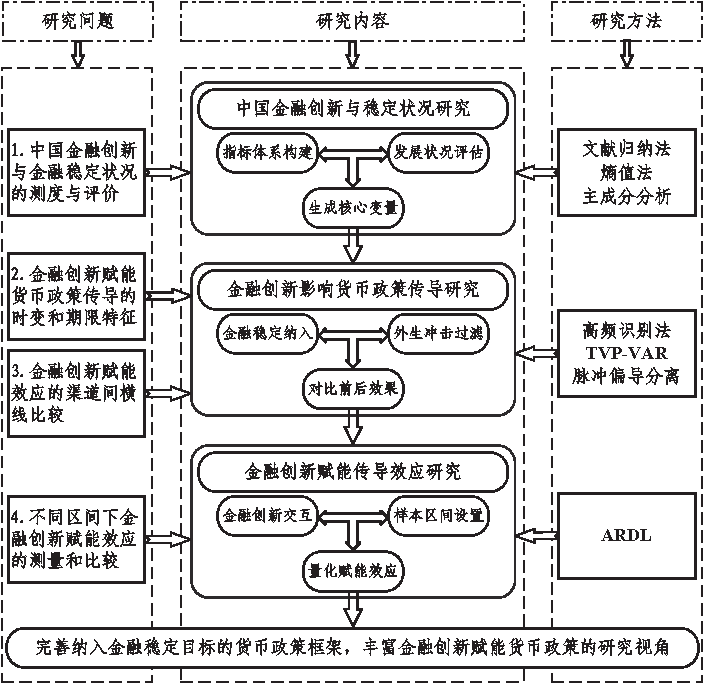
\includegraphics[width=0.4\textwidth]{figures/fig.1-2}
					\caption{技术路线图}
					\label{map}
				\end{wrapfigure}
				\normalsize
				\justifying
				\hspace{2em}
				\textcolor{blue}{1.} 构建衡量中国金融创新与宏观金融稳定的指标体系;\\
				\hspace{2em}
				\textcolor{blue}{2.} 利用时变参数VAR模型刻画货币政策传导全过程,采用脉冲偏导分离技术剥离金融创新的赋能效应;\\
				\hspace{2em}
				\textcolor{blue}{3.} 利用自回归分布滞后模型以及自变量交互项来测度金融创新赋能效应,进一步引入时间虚拟变量划分样本区间,深入比较全面金融监管前后的变化结果。
				\hyperlink{pr}{\beamergotobutton{}}
			\end{frame}
			
			\subsection{研究创新与不足}
			\begin{frame}[label=novelty]
				\frametitle{\makebox[\framewidth]{1.4研究创新与不足
					\hfill\raisebox{-0.65ex}{\vspace*{10mm}
\includegraphics[height=0.1\textheight]{slogo}\hspace{-4mm}}}}
				\vspace{4mm}
				\begin{itemize}
					\item 研究创新
					\hyperlink{pr}{\beamergotobutton{}}
					\begin{enumerate}
						\justifying
						\footnotesize
						\item \textbf{研究视角创新。}从宏观视角考察了中国宏观金融创新水平对货币政策传统渠道传导效率的赋能效应,对比了货币政策对传统目标(经济增长与物价稳定)和宏观审慎目标(金融稳定)的传导。
						\item \textbf{研究方法创新。}(1)手工收集百度指数构建金融创新指标;(2)采用利率互换高频数据识别货币政策外生冲击;(3)将脉冲偏导分离技术应用于TVP-VAR模型,探究赋能效应的时变特征和期限特征;(4)遵循“二步法”,扩展货币政策效果方程。
					\end{enumerate}
				\vspace{0mm}
				\item 研究不足
					\begin{enumerate}
						\justifying
						\footnotesize
						\item \textbf{研究对象不足。}只考虑传统的传导渠道,未考虑与金融稳定目标直接相关的有资产价值渠道(Bernanke \& Gertler, 1989)、风险承担渠道(Borio \& Zhu, 2012)、以及风险转移渠道(Dell'Ariccia et al., 2014)。
						\item \textbf{研究数据不足。}(1)百度指数的时间跨度有限,且存在较多关键词未被搜录;(2)数据缺失背景下的无奈之举(刘少波等, 2021)。
						\item \textbf{研究方法不足。}(1)传统“两步法”的缺陷之一:不大适合于多次建模的结果比较;(2)前沿方法利用的是宏观时间序列和面板数据相结合(尹振涛等, 2023;翟光宇等, 2023)。
					\end{enumerate}
				\end{itemize}
			\end{frame}

			\section{指标体系构建}
			\subsection{中国金融创新的测定}
			\begin{frame}
				\frametitle{\makebox[\framewidth]{2.1中国金融创新的测定
					\hfill\raisebox{-0.65ex}{\vspace*{10mm}
\includegraphics[height=0.1\textheight]{slogo}\hspace{-4mm}}}}
					\justifying
					\footnotesize
%					\vspace*{-3mm}
					\hspace{2em}
					\textcolor{blue}{1.} \textbf{选择依据:}基于盛天翔和范从来(2020)、《径山报告》课题组(2020)的研究,并结合《中国金融科技创新发展指数报告(2018)》《中国金融科技运行报告(2021)》《中国金融科技发展概览创新与应用前沿(2020$\sim$2021)》《中国数字金融创新发展报告(2021)》相关权威报告,同时考虑到百度指数的可获得性;\\
					\hspace{2em}
					\textcolor{blue}{2.} \textbf{指标范围:}涉及从微观服务与技术、中观市场与行业、宏观制度与战略,以及直接搜索共四个层面;\\
					\hspace{2em}
					\textcolor{blue}{3.} \textbf{合成方法:}熵值法。
				\begin{table}
					\centering
					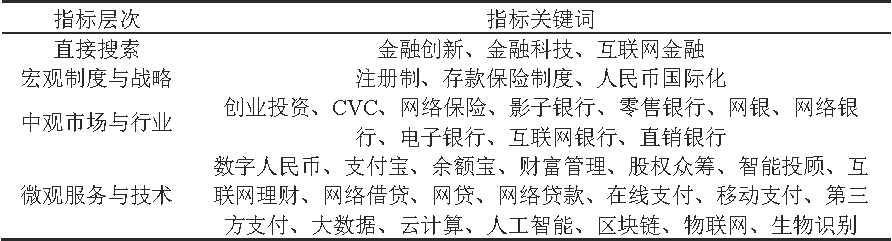
\includegraphics[width=0.7\textwidth]{figures/tab.2-1}
					\caption{金融创新指标关键词选择}
					\label{fi}
				\end{table}
			\end{frame}
			\subsection{中国金融稳定的测定}
			\begin{frame}
				\frametitle{\makebox[\framewidth]{2.2中国金融稳定的测定
					\hfill\raisebox{-0.65ex}{\vspace*{10mm}
\includegraphics[height=0.1\textheight]{slogo}\hspace{-4mm}}}}
				\begin{wraptable}{r}{0.45\textwidth}
					\vspace{-9mm}
					\centering
					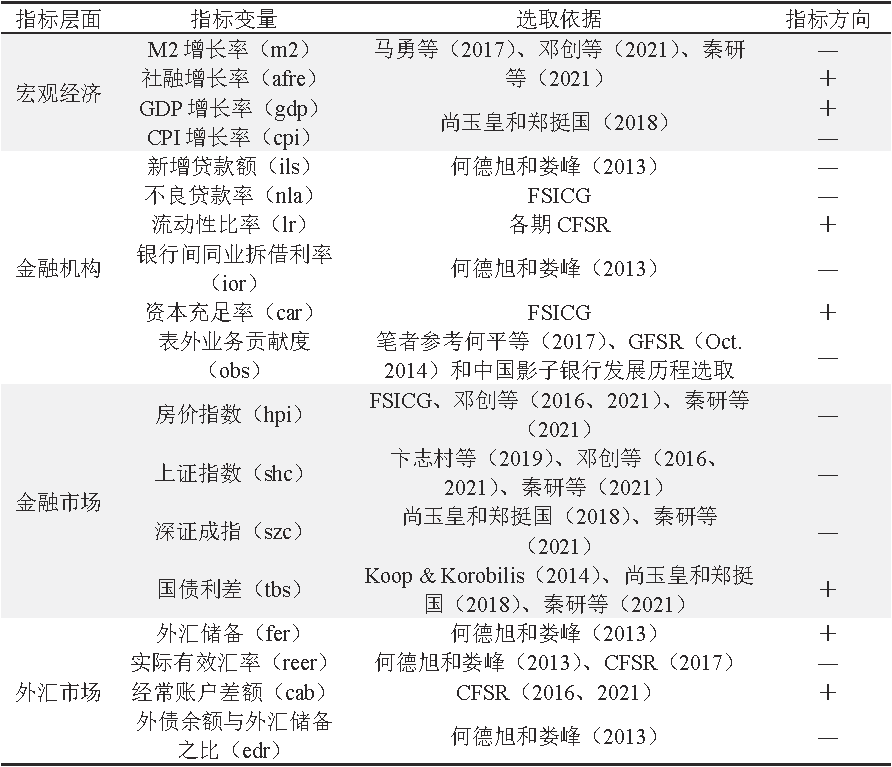
\includegraphics[height=0.75\textheight]{figures/tab.4-3}
					\caption{全国宏观金融稳定指标选择}
					\label{fsi}
				\end{wraptable}
					\justifying
					\vspace*{-3mm}
					\hspace{2em}
					\textcolor{blue}{1.} \textbf{选择依据:}IMF发布的《金融稳健指标编制指南(FSICG)》和《全球金融稳定报告(GFSR)》、中国人民银行发布的《中国金融稳定报告(CFSR)》、何德旭和娄峰(2013)、邓创等(2016、2021)与尚玉皇和郑挺国(2018)等相关研究;\\
					\hspace{2em}
					\textcolor{blue}{2.} \textbf{指标范围:}宏观经济、金融机构、金融市场与外汇市场四个角度出发选取的18个子项指标;\\
					\hspace{2em}
					\textcolor{blue}{3.} \textbf{合成方法:}主成分分析;\\
					\hspace{2em}
					\textcolor{blue}{4.} \textbf{创新:}纳入表外业务贡献度。
			\end{frame}
			\subsection{中国金融创新与金融稳定发展历程}
			\begin{frame}
				\frametitle{\makebox[\framewidth]{2.3中国金融创新与金融稳定发展历程
					\hfill\raisebox{-0.65ex}{\vspace*{10mm}
\includegraphics[height=0.1\textheight]{slogo}\hspace{-4mm}}}}
				\centering
				\begin{minipage}{0.45\textwidth}
					\begin{figure}
						\centering
						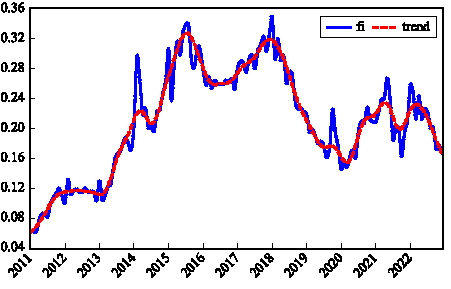
\includegraphics[width=\textwidth]{figures/fig.2-1}
						\caption{金融创新发展历程}
						\label{fi2}
					\end{figure}
				\end{minipage}
				\hspace{5mm}
				\begin{minipage}{0.45\textwidth}
					\begin{figure}
						\centering
						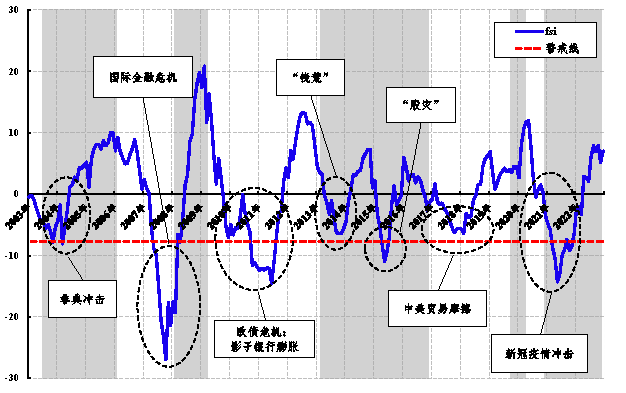
\includegraphics[width=\textwidth]{figures/fig.4-1}
						\caption{金融稳定发展历程}
						\label{fsi2}
					\end{figure}
				\end{minipage}	
			\end{frame}
			
			\section{机制分析与假说提出}
			\subsection{货币政策的传导机制与渠道}
			\begin{frame}
	 			\frametitle{\makebox[\framewidth]{3.1货币政策的传导机制与渠道
					\hfill\raisebox{-0.65ex}{\vspace*{10mm}
\includegraphics[height=0.1\textheight]{slogo}\hspace{-4mm}}}}
				\begin{itemize}
					\justifying
					\item 货币政策传导(机制):\\
					{\normalsize 货币当局通过直接对货币政策工具操作,相应引起数量型或价格型操作目标和中介目标的反应,并通过各种渠道实现货币政策最终目标的传递过程。}
					\item 货币政策传导渠道:\\
					{\normalsize 主要根据金融体系的代表性变量进行划分,如市场利率、资产价格、汇率、银行贷款及其资产负债表等。}
					\item 货币渠道理论
					\item 信贷渠道理论
				\end{itemize}
			\end{frame}
			\subsection{金融创新赋能货币政策传导}
			\begin{frame}
				\frametitle{\makebox[\framewidth]{3.2金融创新赋能货币政策传导
					\hfill\raisebox{-0.65ex}{\vspace*{10mm}
\includegraphics[height=0.1\textheight]{slogo}\hspace{-4mm}}}}
				\begin{enumerate}
					\justifying
					\normalsize
					\item 基于盛松成和翟春(2016)的研究,以余额宝为代表的货币市场基金直销平台,在借助第三方支付、网络借贷、直销银行以及互联网理财等金融创新的共同影响下,极大程度地影响了传统数量型指标的可测性和可控性;
					\item 由于金融创新的隐蔽性,此类金融创新筹集到的资金流向和用途难以在发展初期受到严格的监管;\\
					\item 相反,纳入全面监管的金融创新提高了数据信息的透明度,强化了货币当局对其的有效控制。
				\end{enumerate}
				\centering
				\begin{minipage}{0.8\textwidth}
					\begin{block}{假说一}
						\fangsong 
						\justifying
						\hspace{2em}
						1a:金融创新会降低货币政策向数量型渠道的传导效率。\\
						\hspace{2em}
						1b:纳入监管的金融创新会提高数量型渠道的传导效率。
					\end{block}
				\end{minipage}
			\end{frame}
			\begin{frame}
				\frametitle{\makebox[\framewidth]{3.2金融创新赋能货币政策传导
						\hfill\raisebox{-0.65ex}{\vspace*{10mm}
\includegraphics[height=0.1\textheight]{slogo}\hspace{-4mm}}}}
				\begin{enumerate}
					\justifying
					\normalsize
					\item 基于刘少波等(2021)的研究,商业银行利用金融科技驱动下的金融创新,不仅能够利用结构化信息对客户信用程度进行精准识别,极大缓解信息不对称,还可以将信息抵押化,拓宽信贷业务渠道和潜在客户规模。
					\item 一方面,金融创新的便捷性、普惠性和可获性提升了银行信贷业务的投放规模;
					\item 另一方面,金融创新的安全性和智能化优化了信贷配给和负债经营,进而从整体上赋能了企业和居民获得银行贷款的效率,提高了实体经济部门的生产效率。
				\end{enumerate}
				\centering
				\begin{minipage}{0.7\textwidth}
					\begin{block}{假说二}
						\fangsong 
						\justifying
						\hspace{2em}
						金融创新会强化数量型渠道的产出效应。
					\end{block}
				\end{minipage}
			\end{frame}
			\begin{frame}
				\frametitle{\makebox[\framewidth]{3.2金融创新赋能货币政策传导
						\hfill\raisebox{-0.65ex}{\vspace*{10mm}
\includegraphics[height=0.1\textheight]{slogo}\hspace{-4mm}}}}
				\begin{enumerate}
					\justifying
					\normalsize
					\item 金融科技通过显著促进企业数字化转型(吴非等, 2023),有力发展了数字经济。
					\item 数字经济通过弱化价格粘性而降低了企业投资对于名义利率的敏感性(战明华和卢垚, 2023)。
					\item 因此,在以金融科技为驱动的金融创新发展下,数字技术与传统的实体经济紧密融合,提升了数字化产业对整体价格的调控能力,弱化了价格粘性。
				\end{enumerate}
				\centering
				\begin{minipage}{0.7\textwidth}
					\begin{block}{假说三}
						\fangsong 
						\justifying
						\hspace{2em}
						金融创新会弱化价格型渠道的产出效应。
					\end{block}
				\end{minipage}
			\end{frame}
			
			\subsection{金融创新影响金融稳定目标}
			\begin{frame}[label=theo-flaws]
				\frametitle{\makebox[\framewidth]{3.3金融创新影响金融稳定目标
					\hfill\raisebox{-0.65ex}{\vspace*{10mm}
\includegraphics[height=0.1\textheight]{slogo}\hspace{-4mm}}}}
				\begin{enumerate}
					\justifying
					\normalsize
					\item 基于信息经济学理论,金融交易前后的信息不对称性是市场经济的弊端,危害交易双方利益甚至金融稳定;
					\item 然而,金融创新对逆向选择和道德风险的影响效果并不能简单概括;
					\item 因此,基于信息经济学下金融创新对金融稳定的影响机制应当分类讨论;
					\item 考虑金融创新的不同层面,这对宏观金融稳定目标的影响机制更加复杂,相关理论亟待补充和完善。
					\hyperlink{pr}{\beamergotobutton{}}
				\end{enumerate}
			\end{frame}
			
			\section{模型构建与变量选择}
			\subsection{模型构建与脉冲剥离}
			\begin{frame}
				\frametitle{\makebox[\framewidth]{4.1模型构建与脉冲剥离
					\hfill\raisebox{-0.65ex}{\vspace*{10mm}
\includegraphics[height=0.1\textheight]{slogo}\hspace{-4mm}}}}
				\begin{itemize}
					\item 基准模型\\
					\justifying
					{\normalsize
					给出简化形式SVAR的紧凑表达:
					\vspace{-3mm}
					\[
					y_t=X_t\beta _t+A_{t}^{-1}\varSigma _t\varepsilon _t
					\vspace{-3mm}
					\]
				    相关参数的形式与设定参考Primiceri(2005)和Nakajima(2011)。
					}
					\item 脉冲偏导分离技术
					\begin{itemize}
						\justifying
						\item \textbf{基本思想:}将某一中介变量是否作为内生变量纳入基准模型,通过纳入前后的脉冲响应变化来观测该变量对脉冲响应的“赋能”情况。
						\item \textbf{技术原理:}在测度货币政策的有效性时,除将货币政策工具以外的其他所有变量的即期扰动项自动固定,表现为货币政策扰动项对最终目标变量的脉冲响应。
					\end{itemize}
				\end{itemize}
			\end{frame}
			\subsection{变量选择与数据处理}
			\begin{frame}
				\frametitle{\makebox[\framewidth]{4.2变量选择与数据来源
					\hfill\raisebox{-0.65ex}{\vspace*{10mm}
\includegraphics[height=0.1\textheight]{slogo}\hspace{-4mm}}}}
				\begin{table}
					\centering
					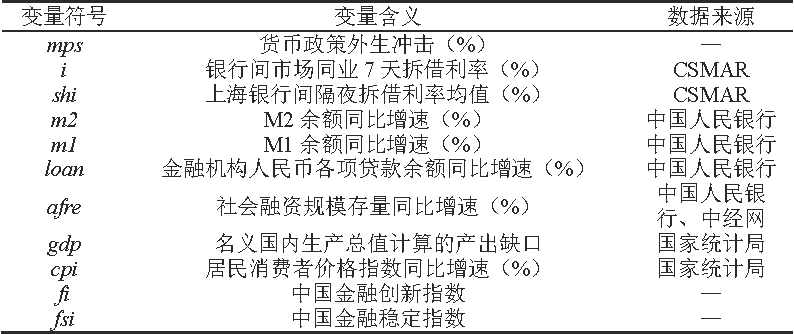
\includegraphics[width=0.8\textwidth]{figures/tab.4-1}
					\caption{变量选择与数据来源}
					\label{data}
				\end{table}
			\end{frame}
			\subsection{货币政策外生冲击的识别}
			\begin{frame}
				\frametitle{\makebox[\framewidth]{4.3货币政策外生冲击的识别
						\hfill\raisebox{-0.65ex}{\vspace*{10mm}
\includegraphics[height=0.1\textheight]{slogo}\hspace{-4mm}}}}
					\begin{itemize}
						\justifying
						\normalsize
						\item \textbf{方法简述:}利用中国人民银行发布重要政策公告前后相邻的两个交易日内的FR007-IRS的日频收盘价格之差作为构造外生冲击($OMP_t$)的原始数据。
						\item \textbf{具体步骤:}
						\vspace{-0mm}
						\[
						OMP_t=IRS_t-IRS_{t,-1}
						\vspace{-0mm}
						\]
						{\footnotesize 利用17个宏观经济金融变量所合成的5个主成分因子($PC_{i,t}$)剔除宏观基本面因素干扰:}
						\vspace{-3mm}
						\[
						OMP_t=\rho _1+\sum_{i=1}^5{\theta _i\times PC_{i,t-1}}+\epsilon _{1t}
						\vspace{-3mm}
						\]
						{\footnotesize 继续剔除货币当局的经济预期影响:}
						\vspace{-3mm}
						\[
						\hat{\epsilon}_{1t}=\rho _2+\delta _1Eiav_t+\delta _2Ecpi_t+\epsilon _{2t}
						\vspace{-2mm}
						\]
						{\footnotesize 那么,货币政策外生冲击就是$\tilde{\hat{\epsilon}}_{2t}$。}
						\item \textbf{相关文献:}Romer \& Romer, 2004; 李云峰和王彦卿, 2016; Paul, 2020; Miranda-Agrippino \& Ricco, 2021; 张成思等, 2022; 陈贞竹等, 2023.
					\end{itemize}
			\end{frame}
			\begin{frame}
				\frametitle{\makebox[\framewidth]{4.3货币政策外生冲击的识别
					\hfill\raisebox{-0.65ex}{\vspace*{10mm}
\includegraphics[height=0.1\textheight]{slogo}\hspace{-4mm}}}}
				\begin{figure}
					\begin{minipage}{0.25\textwidth}
						\centering
						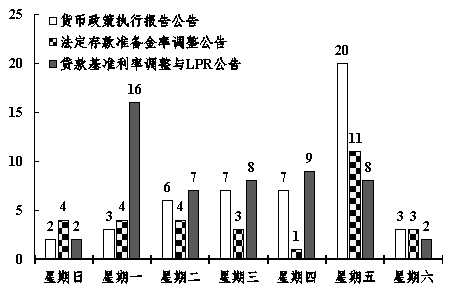
\includegraphics[width=\linewidth]{figures/fig.5-1}
						\caption{中国人民银行重要政策公布时间统计}
						\label{mp}
					\end{minipage}
					\hfill
					\begin{minipage}{0.45\textwidth}
						\centering
						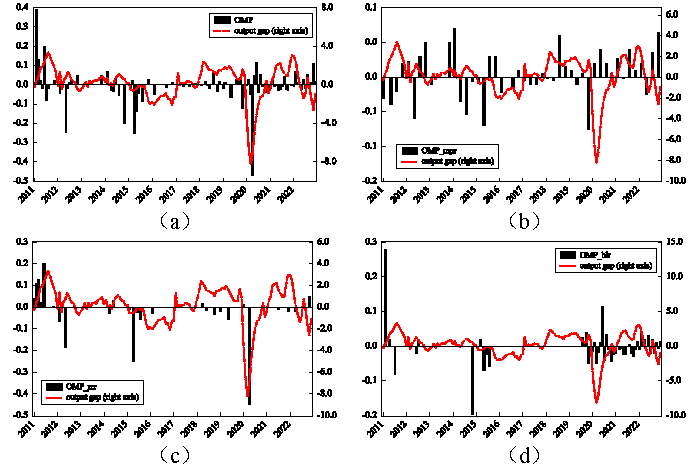
\includegraphics[width=\linewidth]{figures/fig.5-2}	
						\caption{原始货币政策冲击}
						\label{omp}
					\end{minipage}
					\hfill
					\begin{minipage}{0.25\textwidth}
						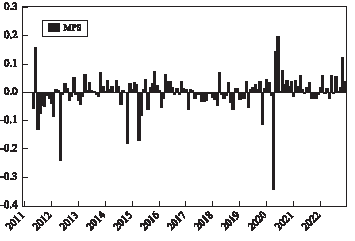
\includegraphics[width=\linewidth]{figures/fig.5-3}	
						\caption{中国货币政策外生冲击}
						\label{mps}
					\end{minipage}
				\end{figure}
			\end{frame}
			
			\section{实证结果分析}
			\subsection{金融创新对货币政策传导的影响}
			\begin{frame}
				\frametitle{\makebox[\framewidth]{5.1赋能效应的时变特征与期限特征
					\hfill\raisebox{-0.65ex}{\vspace*{10mm}
\includegraphics[height=0.1\textheight]{slogo}\hspace{-4mm}}}}
				\begin{itemize}
					\justifying
					\normalsize
					\item \textbf{方法简述:}利用时变参数VAR建模刻画货币政策传导方程,以及脉冲偏导分离技术剥离出金融创新赋能效应。根据模型特点,金融创新的赋能效应具有时变特征和期限特征。
					\item \textbf{时点选择:}利用中国货币政策传导受阻进程中的三个代表性事件节点来重点分析赋能效应,具体为2015M7(社融增速和M2增速的“剪刀差”第一次背离)、2018M3(金融创新指数处于峰值),以及2022M4(“剪刀差”第二次背离)。
					\item \textbf{判断标准:}变量间脉冲响应函数的方向当作判断标准,如果实证结果与理论相一致,则认为该渠道通畅,反之受阻。同理,如果赋能效应的方向与畅通状态相一致,则认为正向赋能,反之逆向“负能”。
				\end{itemize}
			\end{frame}
%			\begin{frame}
%				\frametitle{\makebox[\framewidth]{5.1赋能效应的时变特征与期限特征
%					\hfill\raisebox{-0.65ex}{\vspace*{10mm}
\includegraphics[height=0.1\textheight]{slogo}\hspace{-4mm}}}}
%				\begin{itemize}
%					\item 第一阶段赋能效应
%					\begin{enumerate}
%						\item 信贷渠道
%					\end{enumerate}
%					\vspace{3mm}
%					\begin{figure}
%						\centering
%						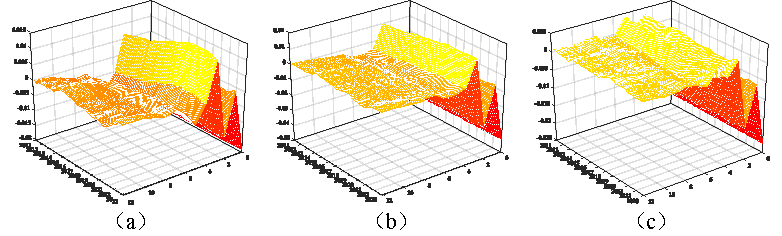
\includegraphics[width=0.7\textwidth]{figures/fig.5-4}
%						\caption{金融创新赋能信贷渠道第一阶段总效应}
%						\label{3D}
%					\end{figure}
%					\vspace{-8mm}
%					\justifying
%					\footnotesize
%					{注:图8a对应的是金融创新赋能前信贷渠道变量对货币政策外生冲击一单位扰动的脉冲响应图像,图8b对应的则是金融创新赋能后的图像,图8c是后者与前者的差值。}
%				\end{itemize}
%			\end{frame}
			\begin{frame}
				\frametitle{\makebox[\framewidth]{5.1赋能效应的时变特征与期限特征
						\hfill\raisebox{-0.65ex}{\vspace*{10mm}
\includegraphics[height=0.1\textheight]{slogo}\hspace{-4mm}}}}
				\begin{wrapfigure}{r}{0.3\textwidth}
					\centering
					\vspace{-5mm}
					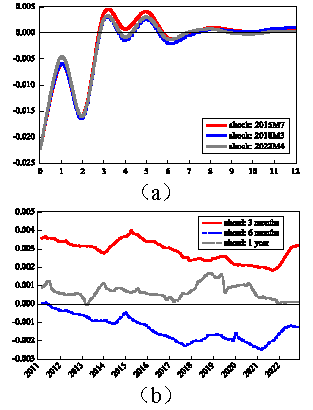
\includegraphics[height=0.7\textheight]{figures/fig.5-5}
				\end{wrapfigure}
					\vspace{-3mm}
					\textcolor{blue}{\footnotesize $\blacksquare$} \large 第一阶段赋能效应\\
					\hspace{1em}
					\textcolor{blue}{\footnotesize 1.} {\normalsize 信贷渠道}\\
					\justifying
					\footnotesize
					\hspace{2em}
					\textcolor{blue}{\tiny $\blacksquare$} 赋能前的第一阶段传导明显受阻,即单位货币政策冲击会造成信贷紧缩;\\
					\hspace{2em}
					\textcolor{blue}{\tiny $\blacksquare$} 对于货币政策传导受阻的三个时点(见图a),金融创新的赋能效应在即期为负,而后不断提升并在第3期左右超过零值,随后上下不断振荡并从第7期始逐渐收敛于零;\\
					\hspace{2em}
					\textcolor{blue}{\tiny $\blacksquare$} 对于三个提前期(见图b),赋能效应曲线存在较大差距;\\
					\hspace{2em}
					\textcolor{blue}{\tiny $\blacksquare$} 总的来看,信贷渠道第一阶段的传导并不畅通,中国金融创新“负能”了这一阶段的传导效率,这种“负能”效应在早期传导受阻时期的弱化更加明显,但在中长期转为正向的赋能效用而且在提前3月的各时点的强化强度最佳。
			\end{frame}
			\begin{frame}
				\frametitle{\makebox[\framewidth]{5.1赋能效应的时变特征与期限特征
					\hfill\raisebox{-0.65ex}{\vspace*{10mm}
\includegraphics[height=0.1\textheight]{slogo}\hspace{-4mm}}}}
				\begin{wrapfigure}[20]{r}{0.3\textwidth}
					\centering
					\vspace{3mm}
					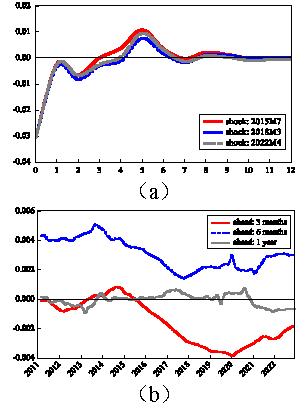
\includegraphics[height=0.7\textheight]{figures/fig.5-6}
				\end{wrapfigure}
				\vspace{-3mm}
				\textcolor{blue}{\footnotesize $\blacksquare$} \large 第一阶段赋能效应\\
				\hspace{1em}
				\textcolor{blue}{\footnotesize 2.} {\normalsize 广义货币渠道}\\
				\justifying
				\footnotesize
				\hspace{2em}
				\textcolor{blue}{\tiny $\blacksquare$} 金融赋能前,广义货币渠道变量对货币政策外生冲击的脉冲响应函数呈现阶段性特征,即前5期的反馈效应为正值,之后则变为负值,这说明短中期的传导相较于中长期更为通畅;\\
				\hspace{2em}
				\textcolor{blue}{\tiny $\blacksquare$} 对于货币政策传导受阻的三个时点(见图a),金融创新的赋能效应在即期为负,而后不断升高并在第3期左右超过零值后持续上升,随后在第7期开始逐渐收敛于零;\\
				\hspace{2em}
				\textcolor{blue}{\tiny $\blacksquare$} 对于三个提前期(见图b),赋能效应曲线差异较大,只有在中期才保持了整体的正值,短期和长期主要为负值,同样说明了金融创新对此渠道的赋能效应有所降低;\\
				\hspace{2em}
				\textcolor{blue}{\tiny $\blacksquare$} 总的来看,广义货币渠道第一阶段的长期传导受阻,中国金融创新在短期内“负能”了这一阶段的传导效率,但在中长期有效改善这一阻塞情况并实现了正向赋能,特别是在提前6月的各时点的强化效应最佳。
%				\textcolor{blue}{\tiny $\blacksquare$}金融创新赋能前,广义货币渠道变量冲击金融稳定的响应函数基本为正,冲击产出的响应函数在中长期为负,冲击通胀的响应函数基本为负;\\
%				\hspace{2em}
%				\textcolor{blue}{\tiny $\blacksquare$}说明中国广义货币渠道金融体系的传导较为阻塞,收缩社会流动性反而无法稳定宏观金融;对实体经济传导均受阻,其中的产出抑制强度超过对通胀的抑制水平;\\
%				\hspace{2em}
%				\textcolor{blue}{\tiny $\blacksquare$}对于金融稳定目标的传递,金融创新的赋能效应在所有滞后期和几乎所有时点中呈现出负值,实现了全阶段的赋能;\\
%				\hspace{2em}
%				\textcolor{blue}{\tiny $\blacksquare$}对于产出目标的传递,金融创新的赋能效应在第3期后不断攀升并在较高水平逐渐收敛,同时在几乎所有的提前期下持续为正;\\
%				\hspace{2em}
%				\textcolor{blue}{\tiny $\blacksquare$}至于通胀目标的传递,金融创新的赋能效应在不同滞后期内差异较大,围绕零值上下波动,中长期逐渐收敛至零。短期的赋能效应与中长期效应差异较大,金融创新对这一渠道这一目标的赋能效应逐步变为“负能”,随着阻塞的持续,越是弱化了对通胀的传递效率,而强化了广义货币的“非中性”。
			\end{frame}
				\begin{frame}
				\frametitle{\makebox[\framewidth]{5.1赋能效应的时变特征与期限特征
						\hfill\raisebox{-0.65ex}{\vspace*{10mm}
\includegraphics[height=0.1\textheight]{slogo}\hspace{-4mm}}}}
				\begin{wrapfigure}[20]{r}{0.3\textwidth}
					\centering
					\vspace{3mm}
					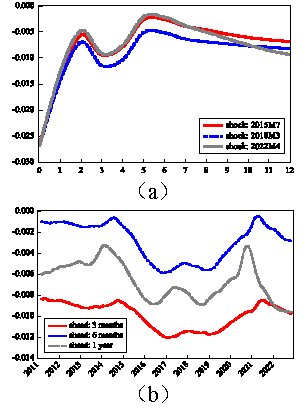
\includegraphics[height=0.7\textheight]{figures/fig.5-7}
				\end{wrapfigure}
				\vspace{-3mm}
				\textcolor{blue}{\footnotesize $\blacksquare$} \large 第一阶段赋能效应\\
				\hspace{1em}
				\textcolor{blue}{\footnotesize 3.} {\normalsize 利率渠道}\\
				\justifying
				\footnotesize
				\hspace{2em}
				\textcolor{blue}{\tiny $\blacksquare$} 金融赋能前,利率渠道变量对货币政策外生冲击的脉冲响应函数同样呈现出阶段性特征,即前2期的反馈效应为正值,之后则变为负值;\\
				\hspace{2em}
				\textcolor{blue}{\tiny $\blacksquare$} 对于货币政策传导受阻的三个时点(见图a),金融创新的赋能效应在即期达到最低值,在全滞后期内保持负值并不收敛于零,其中在2018年3月的赋能效应最低;\\
				\hspace{2em}
				\textcolor{blue}{\tiny $\blacksquare$} 对于三个提前期(见图b),赋能效应曲线在走势上差异不大,而强度上有所差距,但所有曲线在所有时点上保持负值,特别是短期赋能强度最佳,证明金融创新对此渠道的赋能效应十分显著;\\
				\hspace{2em}
				\textcolor{blue}{\tiny $\blacksquare$} 总的来说,利率渠道第一阶段的短期传导受阻,中国金融创新在长中短期均赋能了这一阶段的传导效率,而且赋能强度与广义货币渠道相近,有效疏通了这一阶段,特别是在提前3月的各时点的赋能效应最佳。
			\end{frame}
			\begin{frame}
				\frametitle{\makebox[\framewidth]{5.1赋能效应的时变特征与期限特征
					\hfill\raisebox{-0.65ex}{\vspace*{10mm}
\includegraphics[height=0.1\textheight]{slogo}\hspace{-4mm}}}}
					\begin{itemize}
						\item 第二阶段赋能效应
						\begin{enumerate}
							\item 信贷渠道
							\begin{itemize}
								\justifying
								\item 信贷渠道第二阶段中对通胀目标的传导较为通畅,而对金融稳定和产出目标的传导受阻,中国金融创新有利于这一阶段对实体经济目标以及金融稳定目标的传导。同时,期限特征表示实体经济目标的赋能效应还存在目标间的权衡关系,即对产出的赋能效应超过对通胀目标。
							\end{itemize}
							\item 广义货币渠道
							\begin{itemize}
								\justifying
								\item 广义货币渠道第二阶段中对金融稳定和实体经济目标的传导均有不同程度受阻,中国金融创新不仅有利于这一阶段对产出增长和物价稳定目标的传导,还极大赋能了金融稳定目标的传导。尽管如此,在金融创新赋能的情况下,实体经济目标和金融稳定目标的实现仍然存在权衡关系。
							\end{itemize}
							\item 利率渠道
							\begin{itemize}
								\justifying
								\item 利率渠道第二阶段对金融稳定目标的传导较为通畅,对产出和通胀目标的传导受阻,中国金融创新对这一阶段的实体经济目标均有正向赋能,这是价格型渠道不同于数量型渠道的特殊之处。当然,对各目标的赋能效应仍存在强度上的差异,按量级依次递减。
							\end{itemize}
						\end{enumerate}
						
						\end{itemize}
			\end{frame}
			\begin{frame}
				\frametitle{\makebox[\framewidth]{5.1赋能效应的时变特征与期限特征
						\hfill\raisebox{-0.65ex}{\vspace*{10mm}
\includegraphics[height=0.1\textheight]{slogo}\hspace{-4mm}}}}
				\begin{itemize}
					\item 赋能效应的渠道间比较
					\begin{enumerate}
						\justifying
						\item 中国金融创新具有促进价格型调控转型的鲜明特征,对价格型渠道向实体经济目标的传导均实现了正向赋能,弱化了利率渠道下对实体经济传导所存在的“产出之谜”“价格之谜”,而且赋能强度几乎远超过对数量型渠道的影响;
						\item 金融创新虽不利于货币政策向数量型渠道的传导,但强化了对资金流向的控制,有效稳定数量型渠道维护金融稳定,同时一定程度上促进了产出;
						\item 相较而言,在金融创新的赋能下,传统的货币政策传导渠道和调控方式正积极从数量型向价格型转型过渡,即“价进量退”;
						\item 遗憾的是,金融创新赋能后的利率渠道向实体经济目标的传导仍略有受阻,深化利率市场化改革将是未来的发展方向。
					\end{enumerate}
				\end{itemize}
			\end{frame}
			
			\subsection{金融创新赋能货币政策传导效应的经验证据}
			\begin{frame}
				\frametitle{\makebox[\framewidth]{5.2赋能效应的经验证据
					\hfill\raisebox{-0.65ex}{\vspace*{10mm}
\includegraphics[height=0.1\textheight]{slogo}\hspace{-4mm}}}}
				\begin{itemize}
					\item 金融创新赋能效应的识别
					\begin{itemize}
						\justifying
						\item \textbf{基本思路:}参考Karras(2001)的建模思路,利用分布滞后模型,将金融创新变量纳入货币政策效果方程(Rudebusch \& Svensson, 1999),将所有滞后阶数对应的累计值当作货币政策传导效率的判断对象。
						\item 基准的货币政策效果方程:
						\vspace{-3mm}
						\[
						MPF_{k,t}=\omega +\sum_{l=1}^n{\omega _{1,l}MPF_{k,t-l}+}\sum_{l=0}^n{\omega _{2,l}MPI_{j,t-l}}+\sum_{l=0}^n{\omega _{3,l}MPI_{j,t-l}}\times fi_{t-l}+\varrho _t
						\vspace{-3mm}
						\]
						\item 扩展的货币政策冲击方程:
						\vspace{-3mm}
						\[
						MPI_{j,t}=\kappa +\sum_{l=1}^n{\kappa _{1,l}MPI_{j,t-l}}+\sum_{l=0}^n{\kappa _{2,l}mps_{t-l}}+\sum_{l=0}^n{\kappa _{3,l}mps_{t-l}\times fi_{t-l}}+\zeta _t
						\vspace{-3mm}
						\]
						\item \textbf{进一步研究:}以2020年1月为时间节点作为全面监管的开端,对原交互项再次引入时间虚拟变量($\mathbb{B}$)。
					\end{itemize}
				\end{itemize}
			\end{frame}
			\begin{frame}
				\frametitle{\makebox[\framewidth]{5.2赋能效应的经验证据
						\hfill\raisebox{-0.65ex}{\vspace*{10mm}
\includegraphics[height=0.1\textheight]{slogo}\hspace{-4mm}}}}
				\vspace{5mm}
				\begin{itemize}
					\item 金融创新与货币政策冲击方程
					\begin{itemize}
						\justifying
						\footnotesize
						\item 赋能前,货币政策外生冲击向三大渠道的传导效率方向($\sum{\kappa _{2,j,l}}$)均表现异常,第一阶段的传导均有不同程度的受阻;
						\item 从系数绝对值来看,利率渠道的传导受阻效果相对最小,而数量型渠道传导受阻效果较大且接近;
						\item 金融创新对这一阶段均造成了逆向“负能”,非但没有改变系数累计值的方向,甚至扩大了受阻效果,这一发现与流动性囤积期间的赋能效应相类似;
						\item 不同的是,流动性囤积期间,金融创新对利率渠道第一阶段的长中短各期实现了正向的赋能,有效改善了此时的传导效率。
					\end{itemize}
				\end{itemize}
				\begin{table}
					\centering
					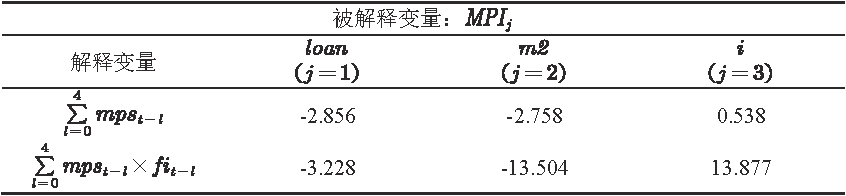
\includegraphics[width=0.55\textwidth]{figures/tab.6-1}
					\caption{金融创新与货币政策冲击方程估计结果}
					\label{tab.6-1}
				\end{table}
			\end{frame}
			\begin{frame}
				\frametitle{\makebox[\framewidth]{5.2赋能效应的经验证据
						\hfill\raisebox{-0.65ex}{\vspace*{10mm}
\includegraphics[height=0.1\textheight]{slogo}\hspace{-4mm}}}}
				\vspace{2mm}
				\begin{itemize}
					\item 金融创新与货币政策效果方程
					\begin{itemize}
						\justifying
						\footnotesize
						\item 金融创新不利于各渠道下第一阶段的传导,但有利于各渠道实现宏观金融稳定;
						\item 金融创新赋能了数量型渠道对产出目标的传导效率,尤其是实现了对广义货币渠道各目标的正向赋能;
						\item 在全样本区间下,金融创新对于利率渠道向产出目标的传导有所抑制;
						\item 中国金融创新不断得到了有益引导,随着利率市场化的不断深入,其对价格型渠道的赋能效应才逐渐彰显,对数量型渠道的削弱也相应增强。
					\end{itemize}
				\end{itemize}
				\begin{table}
					\centering
					\begin{minipage}{0.65\textwidth}
						\centering
						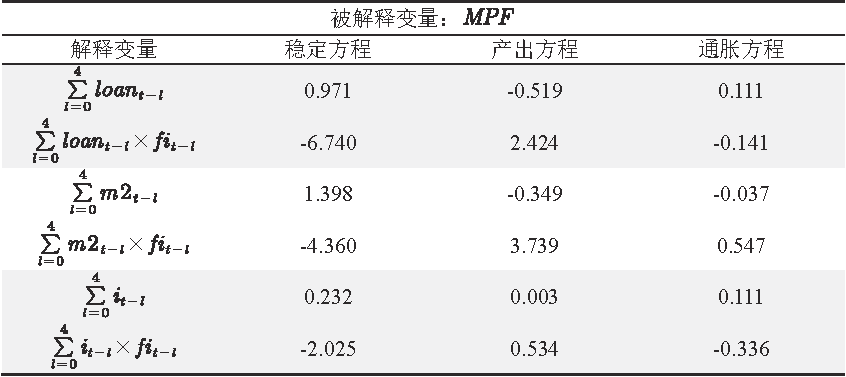
\includegraphics[width=0.8\textwidth]{figures/tab.6-2}
					\end{minipage}
					\hspace{-3mm}
					\begin{minipage}{0.25\textwidth}
						\caption{金融创新与货币政策效果方程估计结果}
						\label{tab.6-2}
					\end{minipage}
				\end{table}
			\end{frame}
			\begin{frame}
				\frametitle{\makebox[\framewidth]{5.2赋能效应的经验证据
						\hfill\raisebox{-0.65ex}{\vspace*{10mm}
\includegraphics[height=0.1\textheight]{slogo}\hspace{-4mm}}}}
				\vspace{5mm}
				\begin{itemize}
					\item 进一步分析:金融创新变化与货币政策冲击方程
					\begin{itemize}
						\justifying
						\footnotesize
						\item 时间虚拟变量与数量型渠道变量和金融创新交互项的累计系数均与未纳入时间虚拟变量的累计系数(代表受阻情景)恰好相反;
						\item 相比于2020年前,2020年后金融创新有效赋能了数量型渠道第一阶段的传导,强化了信贷规模和货币数量的可控性,有利于货币当局对金融市场的调控和政策传导;
						\item 与时变参数VAR结果不同的是,金融创新非但没能在全样本期间强化货币政策对价格渠道的传导,更没有在全面监管后实现正向赋能。
					\end{itemize}
				\end{itemize}
				\vspace{2mm}
				\begin{table}
					\centering
					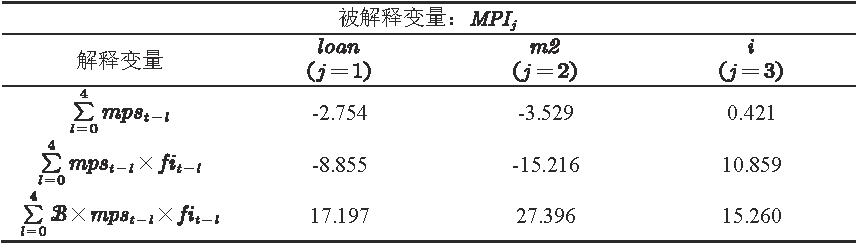
\includegraphics[width=0.55\textwidth]{figures/tab.6-3}
					\caption{金融创新变化与货币政策冲击方程估计结果}
					\label{tab.6-3}
				\end{table}
			\end{frame}
			\begin{frame}
				\frametitle{\makebox[\framewidth]{5.2赋能效应的经验证据
						\hfill\raisebox{-0.65ex}{\vspace*{10mm}\includegraphics[height=0.1\textheight]{slogo}\hspace{-4mm}}}}
				\begin{wraptable}{r}{0.55\textwidth}
					\centering
					\vspace{-10mm}
					\includegraphics[width=0.55\textwidth]{figures/tab.6-4}
					\caption{金融创新变动与货币政策效果方程估计结果}
					\label{tab.6-4}
				\end{wraptable}	
					\justifying
					\hspace{1em}
					\textcolor{blue}{\footnotesize $\blacksquare$} {\large 进一步分析:金融创新变动与货币政策效果方程}\\
					\vspace{2mm}
					\footnotesize
					\hspace{2em}
					\textcolor{blue}{\tiny $\blacksquare$} 伴随全面监管和市场化利率体系的成熟,金融创新强化了数量型渠道向金融稳定目标的传导效率,优化价格型渠道对通胀目标传导的同时恶化了对产出目标的传导;\\
					\hspace{2em}
					\textcolor{blue}{\tiny $\blacksquare$} 纳入监管后的金融创新修复和提升了信贷规模和货币数量的可控性,极大增强了货币政策对数量渠道的传导效率。
				\end{frame}
%				\vspace{5mm}
%				\begin{itemize}
%					\item 进一步分析:金融创新变动与货币政策效果方程
%					\begin{itemize}
%						\justifying
%						\footnotesize
%						\item 伴随全面监管和市场化利率体系的成熟,金融创新强化了数量型渠道向金融稳定目标的传导效率,优化价格型渠道对通胀目标传导的同时恶化了对产出目标的传导;
%						\item 纳入监管后的金融创新修复和提升了信贷规模和货币数量的可控性,极大增强了货币政策对数量渠道的传导效率。
%					\end{itemize}
%				\end{itemize}
%				\begin{table}
%					\begin{minipage}{0.65\textwidth}
%						\centering
%						\includegraphics[width=0.8\textwidth]{figures/tab.6-4}
%					\end{minipage}
%					\hspace{-3mm}
%					\begin{minipage}{0.25\textwidth}
%						\caption{金融创新变动与货币政策效果方程估计结果}
%						\label{tab.6-4}
%					\end{minipage}
%				\end{table}
%			\end{frame}
					
			\section{结论及建议}
			\subsection{研究结论}
			\begin{frame}[label=conclusion]
				\frametitle{\makebox[\framewidth]{6.1研究结论
					\hfill\raisebox{-0.65ex}{\vspace*{10mm}\includegraphics[height=0.1\textheight]{slogo}\hspace{-4mm}}}}
				\begin{enumerate}
					\justifying
					\normalsize
					\item 经济新常态以来,货币当局不断重视维护宏观金融稳定,警惕和防止金融创新通过各渠道造成的系统性风险溢出。中国金融创新疏通了数量渠道对金融稳定目标的传导,强化了信贷规模和货币数量的可控性。
					\item 随着利率市场化改革的深入,利率渠道的相对优势不断彰显。从脉冲响应的强度上看,中国金融创新对利率渠道的赋能效应强于数量渠道,具有促进“量价”转型的鲜明特征。
					\item 中国金融创新对各传统渠道实现产出目标和通胀目标的赋能效应具有明显的推进性。在继续发挥数量渠道相对优势的同时,金融创新强化了利率渠道向通胀传导,而弱化了其产出效应,稳步推动“价进量退”。
					\hyperlink{pr}{\beamergotobutton{}}
				\end{enumerate}
			\end{frame}
			\subsection{政策建议}
			\begin{frame}
				\frametitle{\makebox[\framewidth]{6.2政策建议
					\hfill\raisebox{-0.65ex}{\vspace*{10mm}\includegraphics[height=0.1\textheight]{slogo}\hspace{-4mm}}}}
				\begin{enumerate}
					\justifying
					\item 完善金融监管框架,加强宏观审慎管理,明晰金融创新边界,将金融创新活动全部纳入金融监管当中。
					\item 深化利率市场化改革,疏通价格型传导渠道,做好金融创新顶层设计,促进货币政策向价格调控转型。
					\item 提高形势研判能力,强化多重目标管理,做好成本收益管理,加强货币政策与宏观审慎政策协调搭配。
				\end{enumerate}
			\end{frame}
			%-----------------------
			%       Ending 
			%-----------------------
			\begin{frame}
				\centering
				\Large 感谢专家老师倾听!\\
				欢迎各位批评指正!
				\begin{figure}
					\includegraphics[width=18mm]{logo}
				\end{figure}
				\normalsize 2024年5月26日,南昌
			\end{frame}
		\end{document}
		
